\chapter{Collision Avoidance Implementation}\label{chapter:collisionavoidanceimpl}
In chapter \ref{chapter:collisionavoidance}, we analyze the theoretical aspects of our approach for collision avoidance. We examine in section \ref{sec:closestpoints} how a capsule decomposition and the according closest points between two capsules are sufficiently convex enough to cover the robots collision model. Additionally, we introduce a velocity damping method in \ref{sec:velocitydamping}, which restricts any positive velocity component along the directional vector towards the possible collision center. 

In the previous chapter \ref{chapter:implenv}, we briefly introduced the SoT as a framework and FCL as the according library for proximity queries. This chapter furnishes insights about the implementation of the closest point calculation and velocity damping as entities inside the DG.

Although it can be seen that those two components alone perform well to protect any (self-)collision, in practice there is a need for additional components. There are components needed to operate the robot with a smooth transition of movements. We additionally introduce task definitions for joint velocity and joint position limits as well as a weighting task, which can be used to operate the robot with the necessary safety.

In the following, we have to carefully differentiate the wording between an \textit{entity} and a \textit{task}. Technically speaking, a task denotes an entity inside the DG. Contrary, an entity is not a task, thus it is not able to be pushed on the stack and be considered by the solver.
\newpage
\section{FCL Entity}
As the name might reveal, the FCL entity is responsible for querying proximities based on FCL. We mentioned in the previous section, that during the development of this work, we enhanced FCL with the capsule capabilities. Thus, on startup, we load the capsule parameters such as origin, length and radius from a robot description file\footnote{Unified Robot Description Format(URDF), see \url{http://wiki.ros.org/urdf}}. This parses theses information into a capsule collision object and provides a full collision matrix of all given capsules. 

The collision matrix is represented by output signals for each collision pair. Each output signal provides the closest point from one capsule to another. Hereby, the signals are ordered according to the naming convention \texttt{<capsule-link-1><capsule-link-2>}, which indicates the closest point on the first capsule towards the closest point on the second capsule. Table \ref{tab:collisionmatrix} gives an example for three capsules, namely the right arm, the left arm and the torso. The table shows the resulting output signals. Inside the concrete application, the names are according to the names given in the robot description file.

\begin{table}[width=\textwidth]
\def\arraystretch{3}
\centering
\begin{tabular}{c|c|c|c}
					& 	right-capsule & left-capsule & torso-capsule \\
					\hline
right-capsule & X	& \pbox{4cm}{\texttt{<right-capsule}\\\texttt{left-capsule>}} & \pbox{4cm}{\texttt{<right-capsule}\\\texttt{torso-capsule>}} \\
\hline
left-capsule & \pbox{4cm}{\texttt{<left-capsule}\\ \texttt{right-capsule>}} & X & \pbox{4cm}{\texttt{<left-capsule}\\\texttt{torso-capsule>}} \\
\hline
torso-capsule & \pbox{4cm}{\texttt{<torso-capsule}\\\texttt{right-capsule>}} & \pbox{4cm}{\texttt{<torso-capsule}\\\texttt{left-capsule>}} & X 
\end{tabular}
\label{tab:collisionmatrix}
\caption{Collision Matrix and the produced output signal names.}
\end{table}

This full feature collision matrix might become relatively large, depending on the amount of capsules. This might lead to a large computational cost. At this point however, we only provide output signals inside the DG. With this in mind, the actual proximity computation only gets triggered, when an update of the respective signal is requested by another entity. 
\newpage
\section{Velocity Damping Task}
The implementation of the velocity damping inside a task follows after the FCL entity. We pointed out in the previous chapter \ref{chapter:implenv}, that for defining a task inside the stack, we have to implement a function for the \texttt{Jacobian} and \texttt{error} signal. For convenience, we repeat the inequality formulation of the velocity damping constraint in equation \ref{eqn:taskdampconstraint} here again. 
\begin{equation}
\vec{n}^T\vec{J(p_1,q)} \vec{\dot{q}} \geq - \epsilon \frac{d - ds}{\Delta t}
\end{equation}
In respect of the above equation, we implement the left hand side of the inequality inside the \texttt{Jacobian} function. The right hand side, the velocity boundary, is implemented in the \texttt{error} function. Moreover, we have to specify a set of parameters as input. The equation requires explicitly $\vec{p_1}$, $d_s$ and $\epsilon$ as given, implicitly it also requires $p_2$ to be set for calculating the remaining values such as $d$ and $\vec{n}$.

We will see during the examination of the experiments in chapter \ref{chapter:experiments}, that $d_s$ and $\epsilon$ have to be set as constant input signals as they heavily depend on the robot setup. The two points $\vec{p_1, p_2}$ can be obtained from the FCL entity, as these points are exactly the closest point pair of two collision objects. The connection will be done by plugging the output signals of the FCL entity, into the $\vec{p_1, p_2}$ input signals of the velocity damping task. The Jacobian has to be calculated according to the current joint positions. Our implementation takes the Jacobian with respect to the link origin. This calculation is most often already implemented in various kinematic or dynamic libraries; also inside the SoT. In order to get a Jacobian with respect to the closest point, we apply a twist transformation as explained in section \ref{sec:jacobian}. 

The DG setup for the self-collision avoidance is illustrated in the following graphic \ref{fig:capsuledistance}.
\begin{figure}[h!]
  \centering
    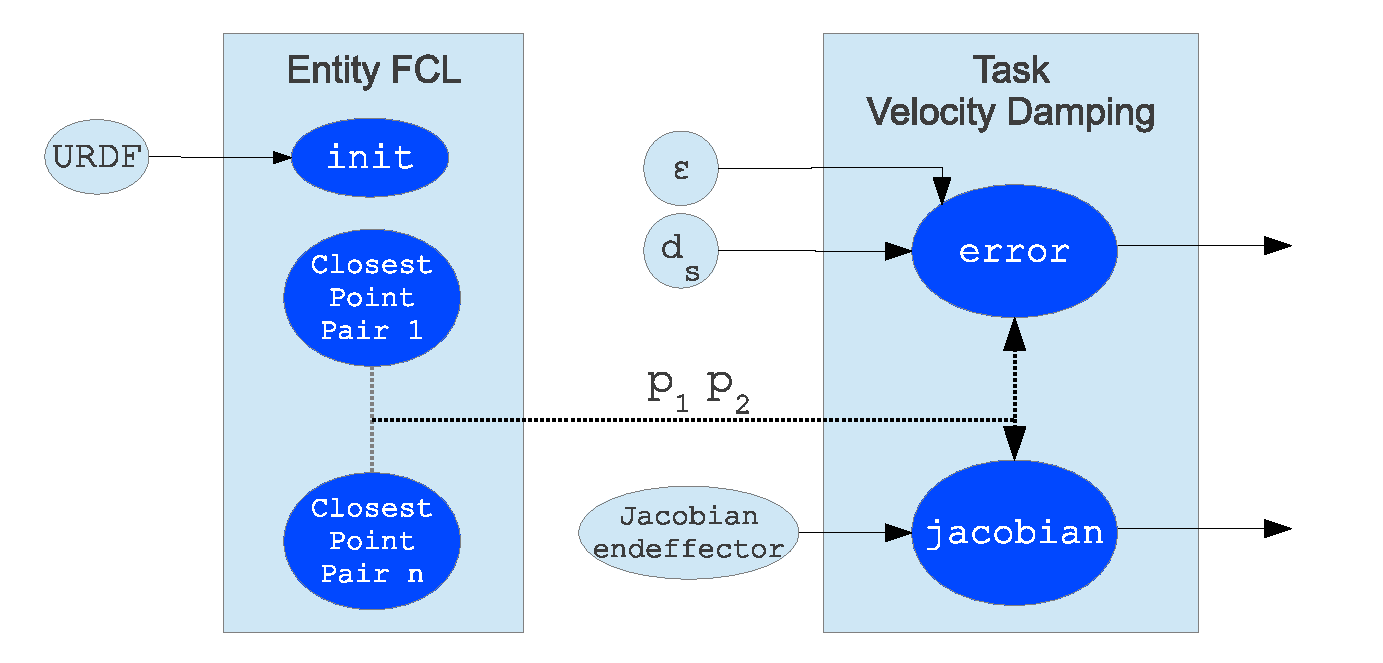
\includegraphics[width=0.8\textwidth]{../figures/dg_collision.eps}
    \caption{Dynamic Graph setup for the self-collision avoidance. EntityFCL provides the closest point pair calculation. These points are plugged into the velocity damping task for calculating $\vec{n}$ and $d$. Values such as $d_s$ and $\epsilon$ are provided as constant signals. Most kinematic or dynamic libraries provide already ways to compute a Jacobian with respect to the end-effector. We provide the end-effector Jacobian as an input signal and apply a twist operation in order to obtain the Jacobian with respect to the closest point. The output signals of the velocity damping are in accordance with the abstract task definition of the SoT, since it requires a \texttt{Jacobian} and \texttt{error} function.}
    \label{fig:capsuledistance}
\end{figure}

We execute only one velocity damping task for avoiding all possible self-collisions. This means, that all collision pairs are on the same level inside the hierarchy. Thus, we configure the task velocity damping to possess multiple input sockets for all closest point pairs and the according control parameters such as $d_s$ and $\epsilon$. This formulation treats all collisions with the same priority.

On the same hand, we only plug the collision pairs we really need to protect the complete robot. This implies an exclusion of adjacent body parts, since they are constantly in collision and would thus violate the solver during the complete execution time. Furthermore, we can exclude collision pairs, which are not able to collide based on the mechanical construction of the robot, such as left and right shoulder. This makes the configuration effort rather simple and the computational complexity is on a minimal.

\section{Joint Limits Task}
The two entities, we described previously, are capable of preventing any self-collision with the robot. However, if we execute only the velocity damping as an exclusive task, we run into trouble as the joint limits might get exceeded. This results in heavy discontinuities which might in the end even destroy the robot. For this purpose of protecting the motors and gears, we introduce two tasks in joint space, which take care about joint position exceeding as well as joint velocity limits. In the generic robot description file, we can calibrate persistent values for the minimal and maximal position for each joint. 

The hierarchical solver inside the SoT operates inside the velocity domain. Thus, for a positioning task, we have to specify a Jacobian matrix, which translates joint space velocities into cartesian space velocities. This formulation allows us to specify the error residual, for example the error between desired and actual position of an end-effector, in cartesian space. \\
At this point, we want to specify a joint space residual, namely the distance between the current joint position and the maximal or minimal boundary. In order to specify this in a similar way, we replace the Jacobian matrix by a simple identity matrix. The task definition then becomes the following:
\begin{equation}
\vec{I} \vec{\dot{q}} \geq \vec{\dot{q}_{err}} \quad \textit{with } \vec{\dot{q}},\vec{\dot{q_{err}}} \in \mathbb{R}^{1\times n}
\end{equation}
where $\vec{I}$ denotes the identity matrix and $\vec{\dot{q_{err}}}$ the error in joint velocity. We have to note here, that the error has to be given in the velocity domain, rather than position. This implies, we have to take the first derivative of the joint position error. Thus the above formulation turns into
\begin{equation}
\vec{I} \vec{\dot{q}} \leq \frac{\vec{q_{max}-q}}{\Delta t} \quad \textit{with } \vec{q_{max}},\vec{\dot{q}} \in \mathbb{R}^{1\times n}
\end{equation}
where $\vec{q_{max}}$ specifies the maximal joint position. $\Delta t$ denotes the time between two computation cycles, which we use to compute a first numerical derivative between two joint positions in time. We enhance this formulation with an additional control gain $k$ to ease any recalibration on runtime. The final equation formulation is presented in equation \ref{eqn:jointlimit}
\begin{eqnarray}\label{eqn:jointlimit}
\vec{I} \vec{\dot{q}} &\leq& \frac{\vec{q_{max}-q}}{k \Delta t}  \notag \\
\vec{I} \vec{\dot{q}} &\geq& \frac{\vec{q_{min}-q}}{k \Delta t}
\end{eqnarray}
We have to point out, that $k$ is placed in the denominator. This has the meaning, that an increase of $k$ leads to an decrease of maximal joint position changes. We implement the joint position limits as a double bounded task, restricting the joint position in the lower and upper boundary. 

The above formulation prevents the solver to resolve any joint state vector $\vec{q}$, which would exceed any joint positions. However, it does not take the joint velocity into considerations. Image equation \ref{eqn:jointlimit} with a low value for $k$ and a current joint position vector $\vec{q}$, which is in the middle of the position limits. There can be situations, where the resulting allowed velocity $\vec{\dot{q}}$ might be too high for the motors. On the same hand, restricting the velocity with a rather big value for $k$ also shrinks down low velocities.

Based on the above considerations, we implement a velocity clamping on top of it. Hereby, in the robot description file, we further specify a maximal joint velocity value. With this, we execute the joint limits with the above formulation, however check if the resulting boundary, the right hand side of the inequality, exceeds the maximal velocity. The task definition looks like the following:

\begin{eqnarray}
\vec{I} \vec{\dot{q}} &\leq& \left\{
\begin{array}{l l}
\frac{\vec{q_{max}-q}}{\Delta t}  & \text{ if } \vec{\dot{q_{err}}}\leq \vec{\dot{q}_{max}} \\
\vec{\dot{q}_{max}} & \text{else}
\end{array} \right. \notag \\
\vec{I} \vec{\dot{q}} &\geq& \left\{
\begin{array}{l l}
\frac{\vec{q_{min}-q}}{\Delta t}  & \text{ if } \vec{\dot{q_{err}}}\leq \vec{\dot{q}_{min}} \\
\vec{\dot{q}_{min}} & \text{else}
\end{array} \right.
\end{eqnarray}
\newpage
\section{Joint Weighting Task}
Finally, we introduce a task, which restricts the movement of expensive joints such as the torso. This task is not necessarily a requirement for safe operations with the robot. It is more a task, which limits the movement of heavy torques and inertia. It further improves the workspace of the robot, since a weighting of the torso means a lower movement of the most commonly shared part of the kinematic chain. The torso will be shared between the head and both arms. However, those tasks of positioning head and arms might be in different priority level such that the torso almost exclusively respects the highest of those tasks. We can correct this by weighting the torso, which is getting compensated by foster a larger movement of different joints, e.g. in the respective arms.

We can easily formulate this task again in joint space. In contrast to the pure identity matrix, we multiply a diagonal weighting matrix with entries according to the inertia of the robot. As we try to minimize the movement as much as possible, we set the resulting velocity to zero.  
\begin{equation}
\vec{W} \vec{I} \vec{\dot{q}} = 0 \quad \text{with } \vec{W} \in \mathbb{R}^{n \times n}
\end{equation}

The equation successfully limits the movement according to the value set on the main diagonal of the weighting matrix. However, when we look at this formulation inside the stack, this approach has some limitations. When we set this task as a rather high priority, the robot does not move. It is clear, that when this task will be fully solved, all DoF are getting used and there is no nullspace for lower priority tasks. With this in mind, we have to set this weighting task always at the least priority position, in order to minimize the velocities. The optimization is done according to the weights as much as possible, yet not restricting any other tasks.


